\chapter{Arquitetura e Funcionamento do Sistema}

Como delineado as tecnologias no capítulo anterior, aqui se apresenta a
arquitetura, demonstrando como todas as tecnologias apresentadas acima se
conectam e conversam entre si.

\begin{figure}[h]
\centering
\caption{Arquitetura e elementos do Sistema}
\label{fig:arch}
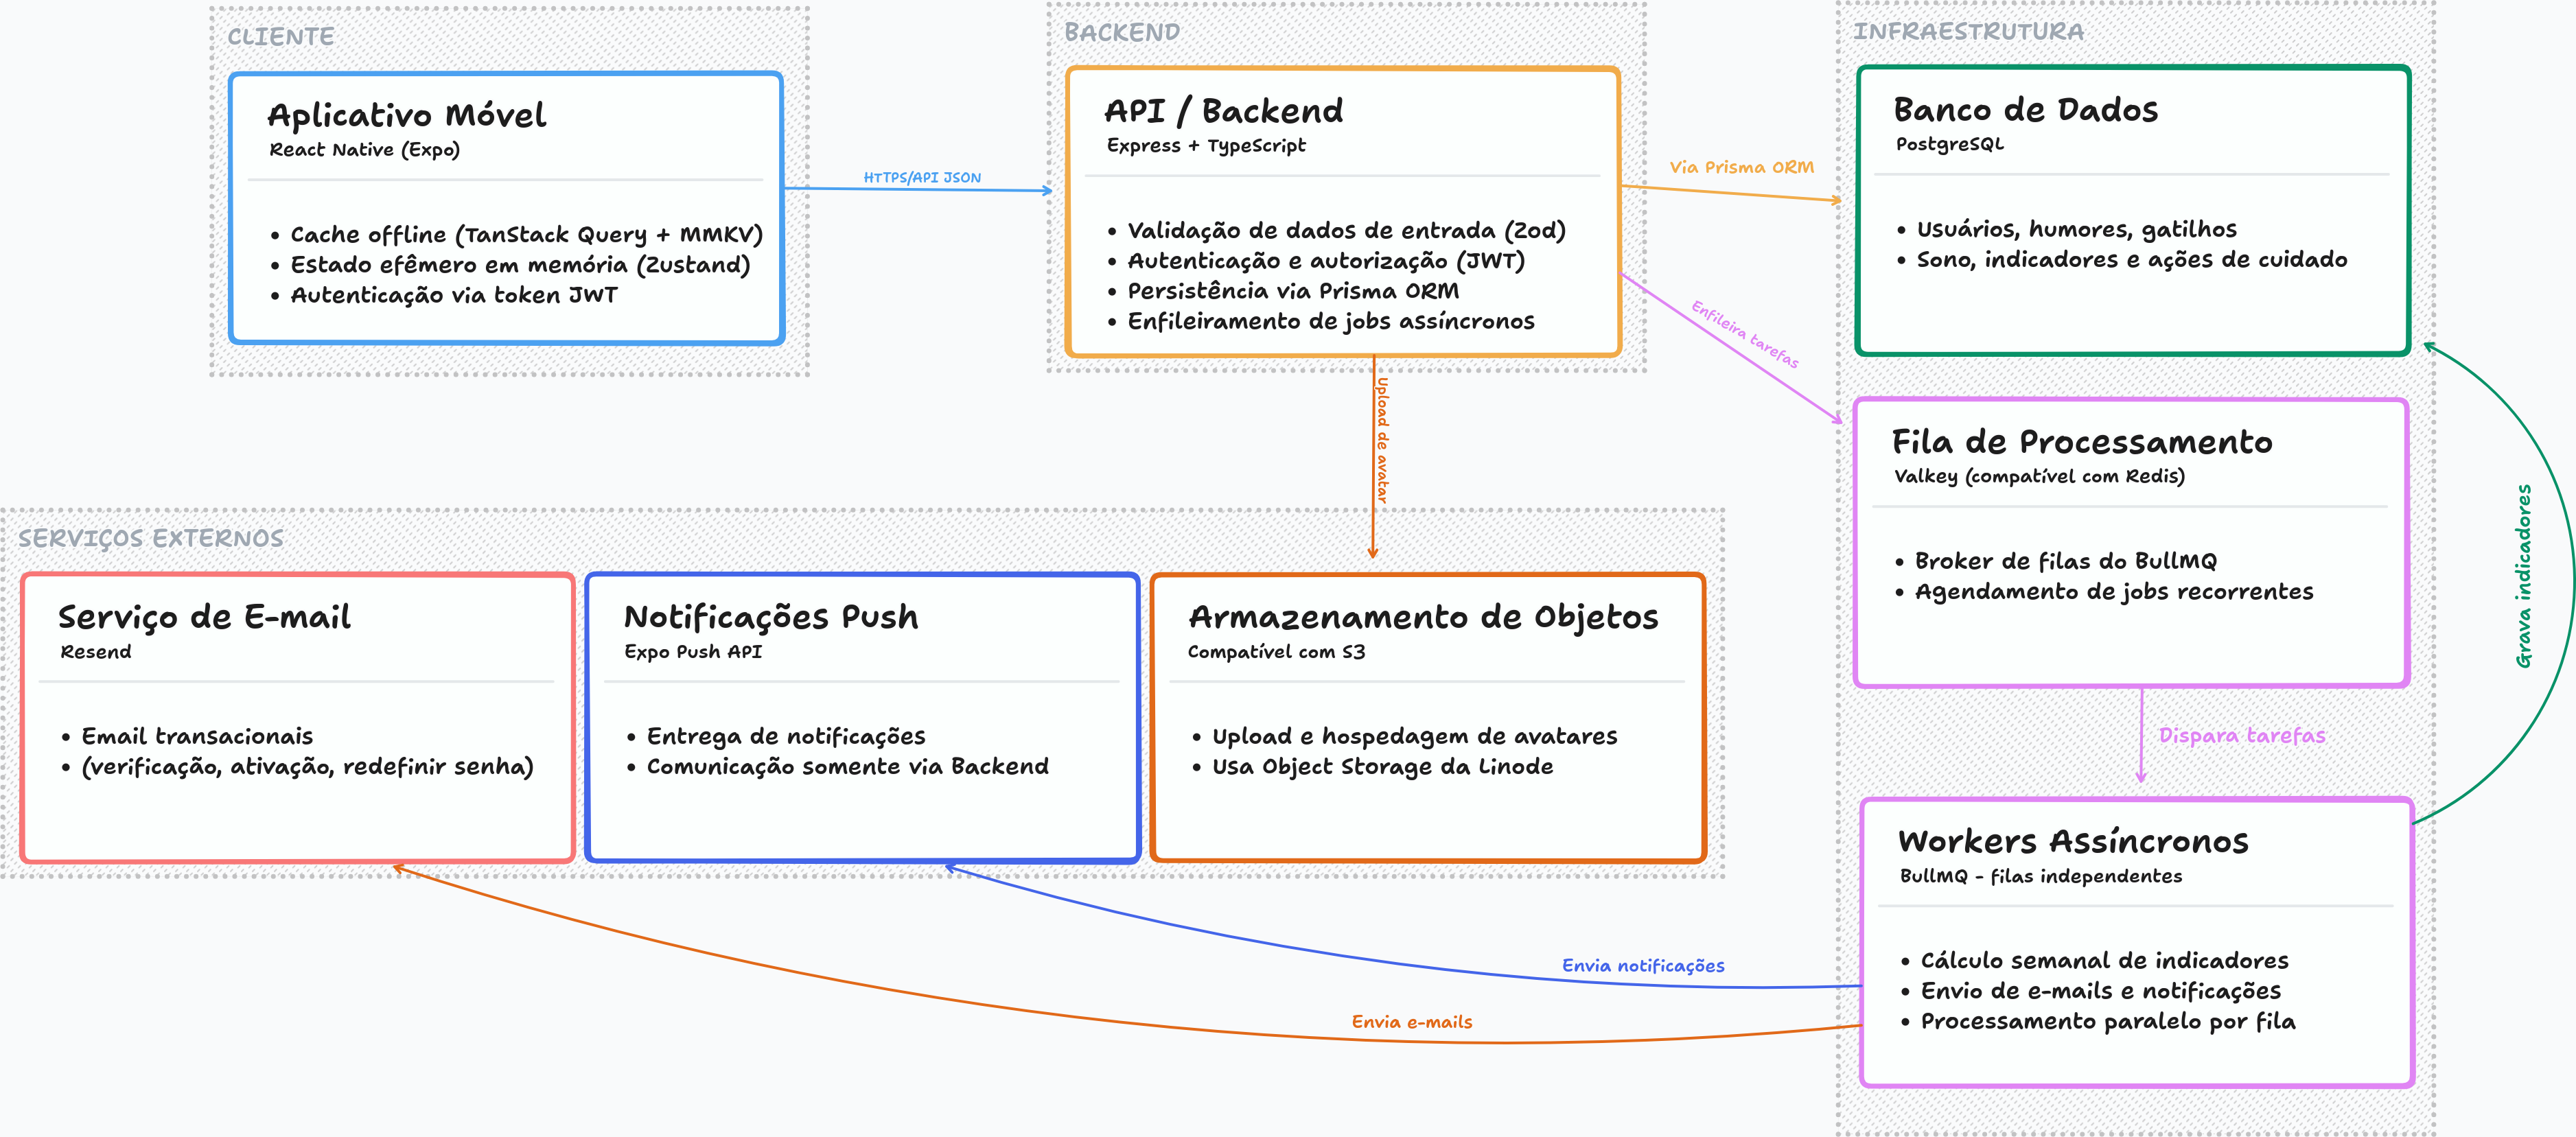
\includegraphics[width=0.9\linewidth]{arch-v2.png}
\source{Elaborado pelo autor (2026)}
\end{figure}

Três planos compõem a arquitetura representada na Figura~\ref{fig:arch} ---
cliente, \textit{back-end} e infraestrutura ---, lidos da esquerda para a
direita. O aplicativo móvel comunica-se exclusivamente com a API por
HTTPS/JSON e mantém no dispositivo apenas o estado efêmero da interface e um
cache local dos dados já consultados; validação, autorização e regras de
domínio ficam concentradas no servidor. A API é a única porta de entrada para
os dados: acessa o PostgreSQL por meio do Prisma, grava avatares no
armazenamento de objetos e delega o trabalho que não precisa bloquear a
resposta ao usuário a filas no Valkey, consumidas por \textit{workers}
independentes. São esses \textit{workers} que enviam e-mails e notificações e
recalculam os indicadores, mantendo a API livre de tarefas de longa duração.

Essa organização tem como principal força a separação de responsabilidades em
torno de um contrato único: como o cliente só conhece a API, mudanças internas
no banco, nas filas ou nos serviços externos não o afetam, e a autenticação por
JWT permite que a API permaneça sem estado, reiniciável sem perda de sessão. O
desacoplamento por filas também torna o registro de um humor uma operação
curta, independente do custo de recalcular indicadores ou disparar
notificações. Em contrapartida, a topologia é deliberadamente monolítica e
vertical: todos os componentes são implantados em um único servidor por meio do
Docker Compose, sem replicação horizontal da API ou separação física entre
banco, fila e \textit{workers}. Isso significa que o trabalho pesado dos
\textit{workers} compete por CPU e memória com o atendimento das requisições, e
que a disponibilidade do conjunto equivale à disponibilidade desse único
\textit{host}. Trata-se de um \textit{trade-off} coerente com o porte do
projeto, mas que delimita seu principal limite de escalabilidade.

Este capítulo detalha o funcionamento de algumas funcionalidades
desenvolvidas durante o projeto. Apenas algumas funcionalidades mais
chaves são abordadas neste capítulo, como o registro de humor, o vínculo
de um gatilho, o histórico consolidado, os indicadores, o registro de
atividades e, por fim, a exportação de dados e a geração de relatórios.

\section{Processo de Login}

Logo ao abrir o aplicativo, o usuário é redirecionado para a tela de
login. A tela em si é relativamente simples, e contém os campos de
email e senha. Existe aqui um elemento proposital: uma forma de
garantir um certo nível de anonimato, em que o usuário não precisa se
identificar com um nome ou número de telefone, tampouco ativar a conta
através de uma plataforma de terceiro, como Google ou Facebook.

Isso se dá, em especial, por dois motivos. Primeiro, o uso de uma tecnologia de
autenticação, como por exemplo, \textit{OAuth} \cite{Hardt:2012} exigiria uma
conexão com plataformas de terceiro, que poderiam então rastrear quais usuários
têm acesso a qual aplicativo --- algo que é fartamente documentado na literatura
sobre os mecanismos usados por tais plataformas para rastrear e monitorar o
acesso a dados de usuários, com o fim de vender e monetizar essas informações.

Essa preocupação não é hipotética: um estudo que interceptou o tráfego de rede
de 36 dos aplicativos mais populares de saúde mental (depressão e cessação de
tabagismo) encontrou transmissão de dados a pelo menos um terceiro em 92\%
deles, sendo que 81\% enviavam dados especificamente a serviços operados por
Google ou Facebook --- e apenas 59\% desses casos declaravam esse
compartilhamento em política de privacidade \cite{Huckvale2019}.

Um estudo posterior, focado exclusivamente em 27 aplicativos de saúde
mental mais populares da Google Play Store, confirmou o mesmo padrão e
o caracterizou formalmente como uma ameaça:

\begin{quote}
  A maioria dos aplicativos representa ameaças relacionadas à rastreabilidade,
  à identificação e à detecção. Isso constitui um risco, pois  alguns terceiros
  podem rastrear, reidentificar e detectar as ações e os dados dos usuários. A
  falta de conscientização também está relacionada a essas ameaças, uma vez que
  os aplicativos não explicam (por exemplo, na política de privacidade) os
  riscos que a publicidade direcionada representa para pessoas com problemas
  mentais, bem como o risco de reidentificação e divulgação de condições de
  saúde mental (por exemplo, ansiedade, depressão).
  \cite[p.~3, tradução nossa]{Iwaya:22}
\end{quote}

Como os próprios autores resumem, a mera vinculação de um usuário a um
aplicativo de saúde mental já pode revelar que essa pessoa possui uma condição
psicológica --- seja ansiedade, depressão, ou, no caso de um aplicativo como o
Nexo, Transtorno Afetivo Bipolar ---, tornando usuários desses aplicativos
particularmente vulneráveis a esse tipo de exposição \cite{Iwaya:22}.

No caso do Nexo, essa cadeia de inferência é especialmente
sensível: a presença do aplicativo na lista de apps instalados de um usuário,
associada ao seu identificador publicitário, permitiria a uma plataforma como a
Meta inferir uma possível condição de saúde mental do usuário para fins de
segmentação de anúncios, sem que este tenha conhecimento ou consentimento
explícito disso.

Segundo, e retomando a proposta de oferecer ao usuário a possibilidade
de \textit{self-service}, aquele que decidisse manter uma instância
própria do aplicativo não precisaria de uma conta em uma plataforma de
terceiro, nem se cadastrar nelas.

\begin{figure}[H]
\centering
\caption{Tela de login}
\label{fig:screenshot-login}
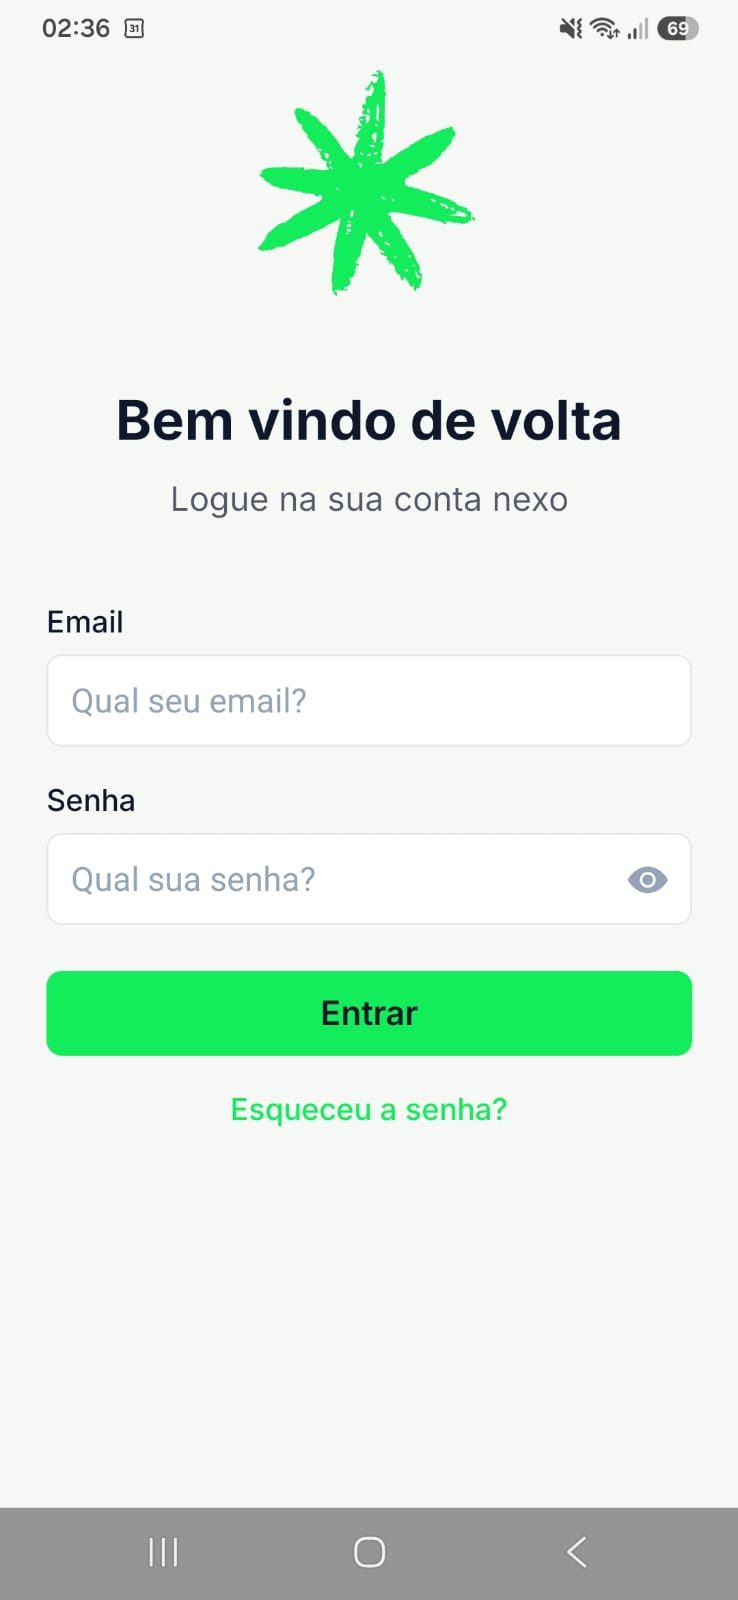
\includegraphics[width=0.70\textwidth,height=0.60\textheight,keepaspectratio]{screenshot-login.jpeg}
\source{Elaborado pelo autor (2026)}
\end{figure}

Por fim, destaca-se aqui que, conforme mencionado anteriormente na
modelagem de casos de uso (figura \ref{fig:use-cases}), ao realizar o
login pela primeira vez é enviado um email com um código de
verificação, seguindo a lógica dos \textit{magic links}. Isso adiciona
uma camada extra de segurança, garantindo que apenas o usuário que
solicitou o login possa acessar a conta.

\section{Página de Consulta de Registros}

A tela inicial é a tela nomeada apenas como ``Novo''. A proposta aqui
é ser a tela de cadastro rápido de um humor, e também é a tela que
visualmente mais destoa das demais. O usuário é apresentado com três
seções distintas:

\begin{itemize}
    \item Cadastro rápido de um humor
    \item Entre ontem e hoje
    \item Registros recentes
\end{itemize}

Respectivamente: uma seção em que o usuário é convidado a ``escolher
um humor'' e iniciar o processo de registro de uma nova entrada; a
seção em que são apresentados os indicadores de nível de energia
acumulado entre o dia anterior e o dia atual, além da média de sono do
dia comparada com a do dia anterior; e, por fim, a listagem dos dez
últimos registros de humor cadastrados pelo usuário.

\begin{figure}[H]
\centering
\caption{Tela de Consulta de Registros}
\label{fig:screenshot-consulta-registros}
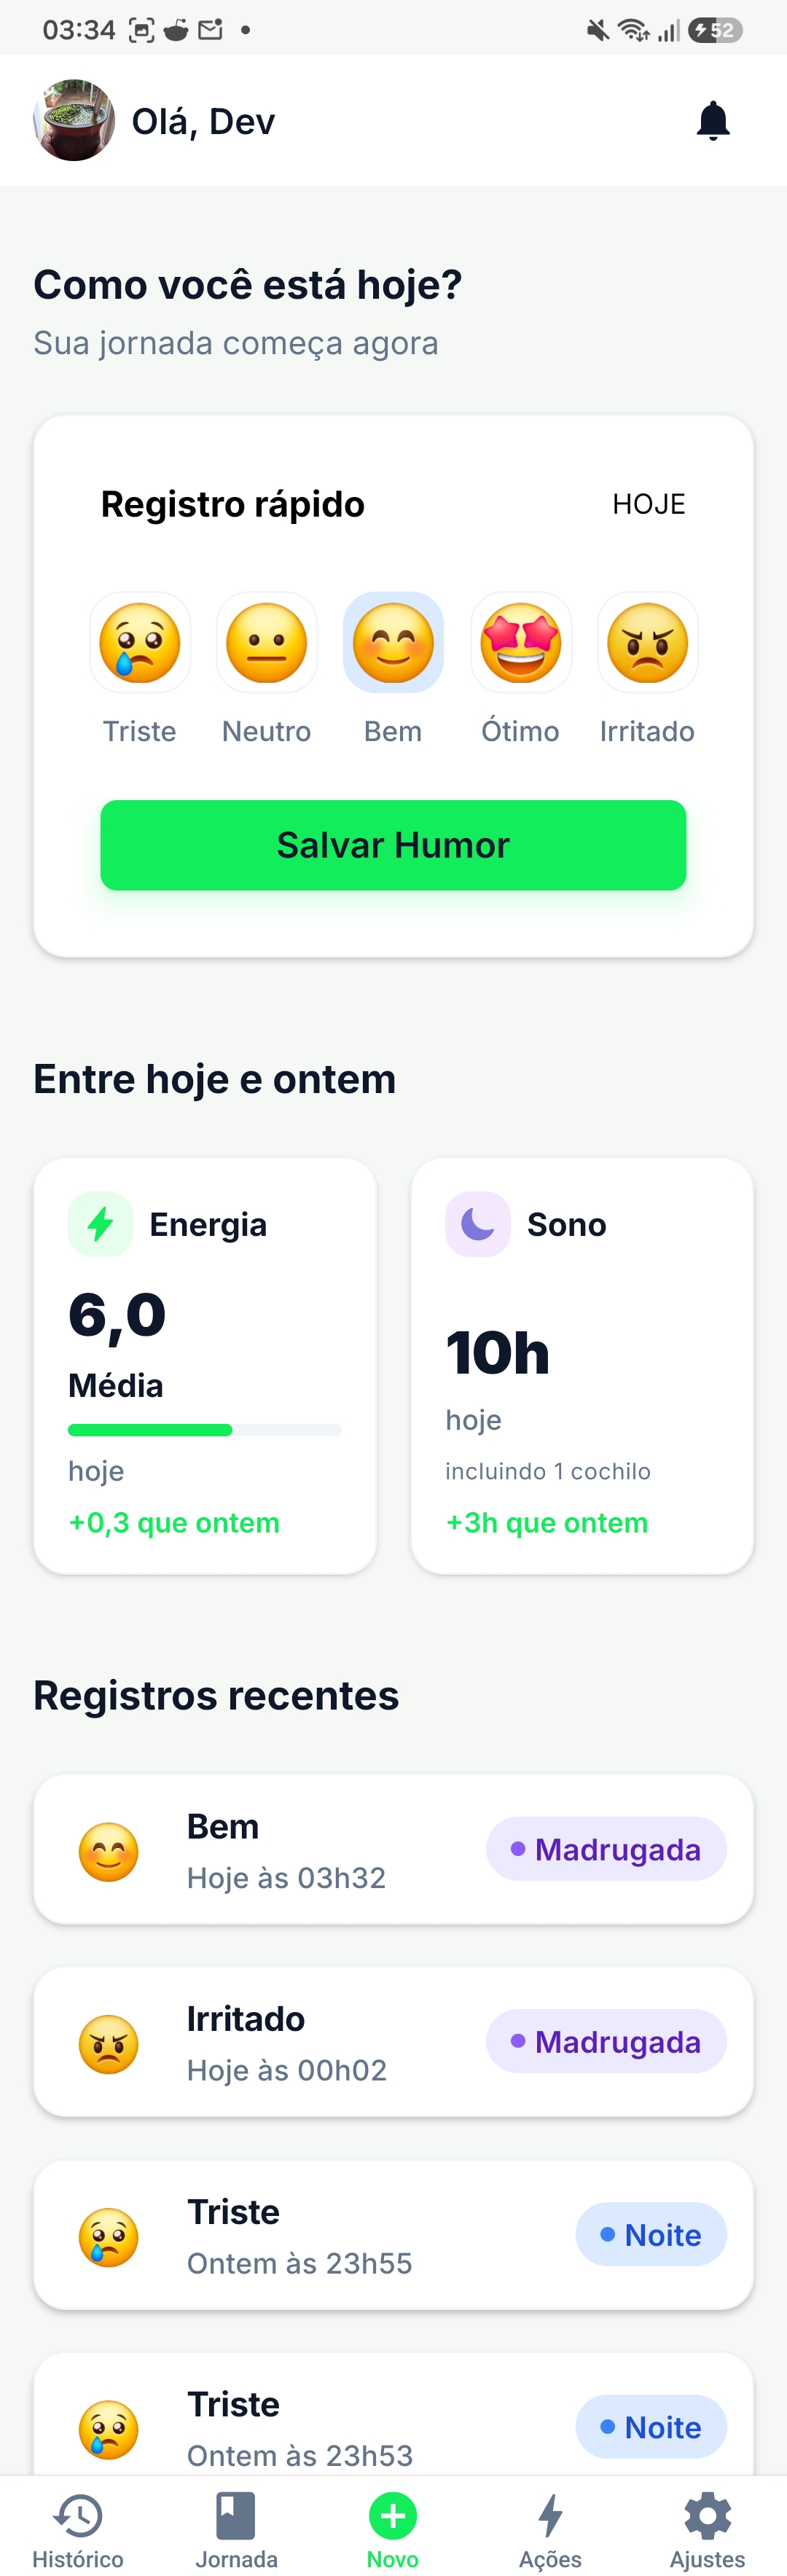
\includegraphics[width=0.70\textwidth,height=0.60\textheight,keepaspectratio]{screenshot-initial-page.jpeg}
\source{Elaborado pelo autor (2026)}
\end{figure}

Aqui já é introduzido ao usuário um padrão de organização e hierarquia:
todos os elementos centrais são organizados em \textit{cards}, exibidos
em no máximo duas colunas. Também é introduzido, caso o usuário já
possua registros de humor cadastrados, o padrão pelo qual esses
registros são resumidos em todas as seções do aplicativo: geralmente
um ícone, um título e alguma informação adicional em destaque.

\section{Criação de Registros de Humor}

Nesta seção, o usuário pode criar novos registros de humor, escolhendo
entre uma lista de opções pré-definidas. O humor selecionado na tela
anterior é mostrado aqui, e o usuário é convidado a julgar, em uma
escala de 1 a 10, como se sente em relação aos níveis de energia,
estresse e ansiedade, respectivamente.

\begin{figure}[H]
\centering
\caption{Criação de Registros de Humor}
\label{fig:screenshot-consulta-humor}
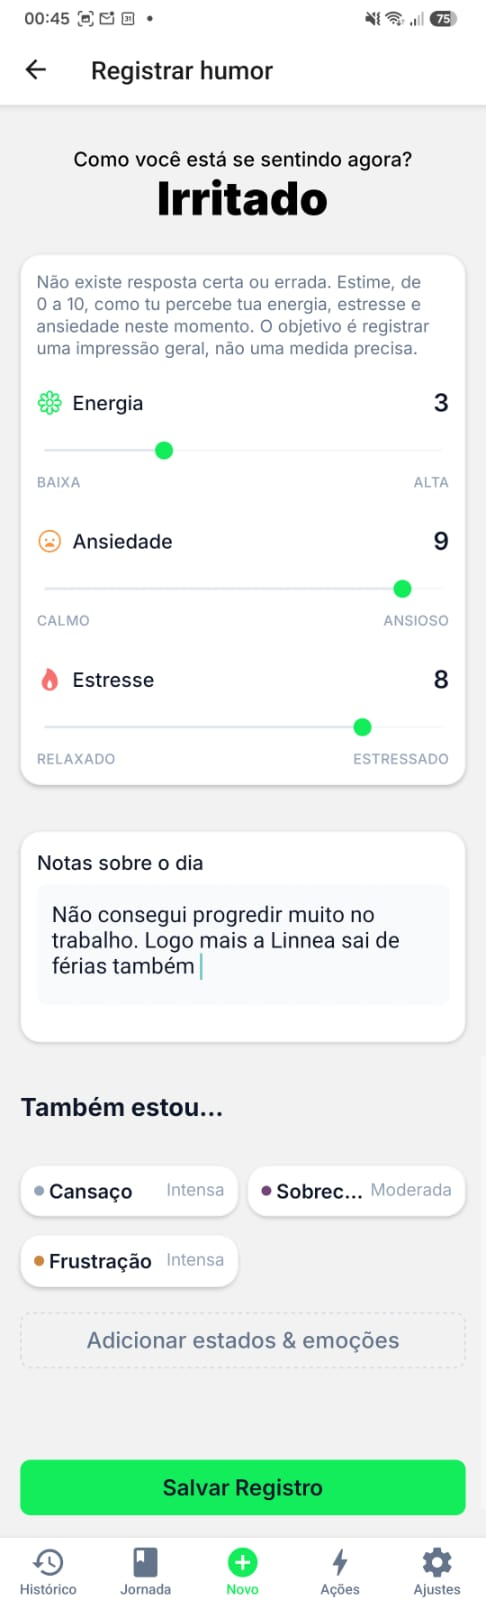
\includegraphics[width=0.70\textwidth,height=0.60\textheight,keepaspectratio]{screenshot-create-mood.jpeg}
\source{Elaborado pelo autor (2026)}
\end{figure}

Naturalmente, é uma questão difícil de responder --- e, como o próprio
aplicativo procura deixar claro, é importante que seja um momento
reflexivo, não necessariamente preciso.

O usuário pode adicionar uma anotação sobre aquele registro em
específico, padrão que se repete em outras telas do aplicativo.

Por fim, o usuário pode escolher o que compõe aquele registro, ou
seja, selecionar emoções e estados/sentimentos que sente naquele
momento. É apresentada uma listagem mista desses elementos, na qual o
usuário seleciona os que mais se aplicam a ele e atribui um nível de
intensidade para cada um. Aqui a escala é menor e mais simples, visando
facilitar a escolha e o julgamento do usuário, entre ``Leve'',
``Moderado'' e ``Intenso'', conforme a figura
\ref{fig:screenshot-add-components}.

\begin{figure}[H]
\centering
\caption{Adicionando sentimentos/emoções}
\label{fig:screenshot-add-components}
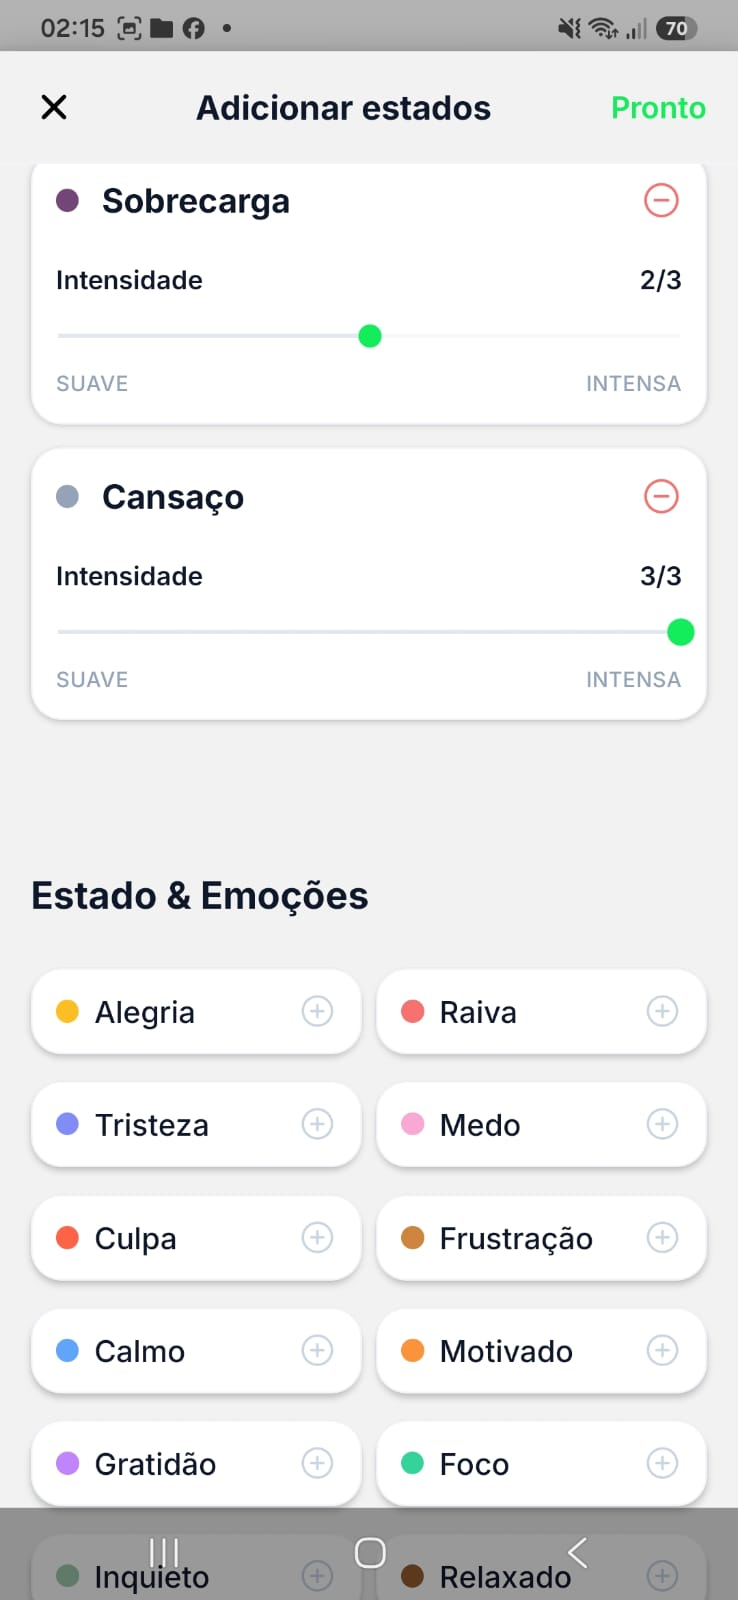
\includegraphics[width=0.70\textwidth,height=0.60\textheight,keepaspectratio]{screenshot-add-components.jpeg}
\source{Elaborado pelo autor (2026)}
\end{figure}

Ao concluir esse processo e salvar, é apresentada ao usuário uma tela
de confirmação, na qual ele pode, opcionalmente, vincular o registro a
um gatilho específico --- que pode ter ocorrido antes de ele salvar o
registro --- ou criar um novo gatilho. O projeto novamente se ancora no
EMA, enriquecendo o registro de humor com mais contexto sobre o que
aconteceu.

\begin{figure}[H]
\centering
\caption{Vinculando um humor com um gatilho}
\label{fig:screenshot-link-mood-trigger}
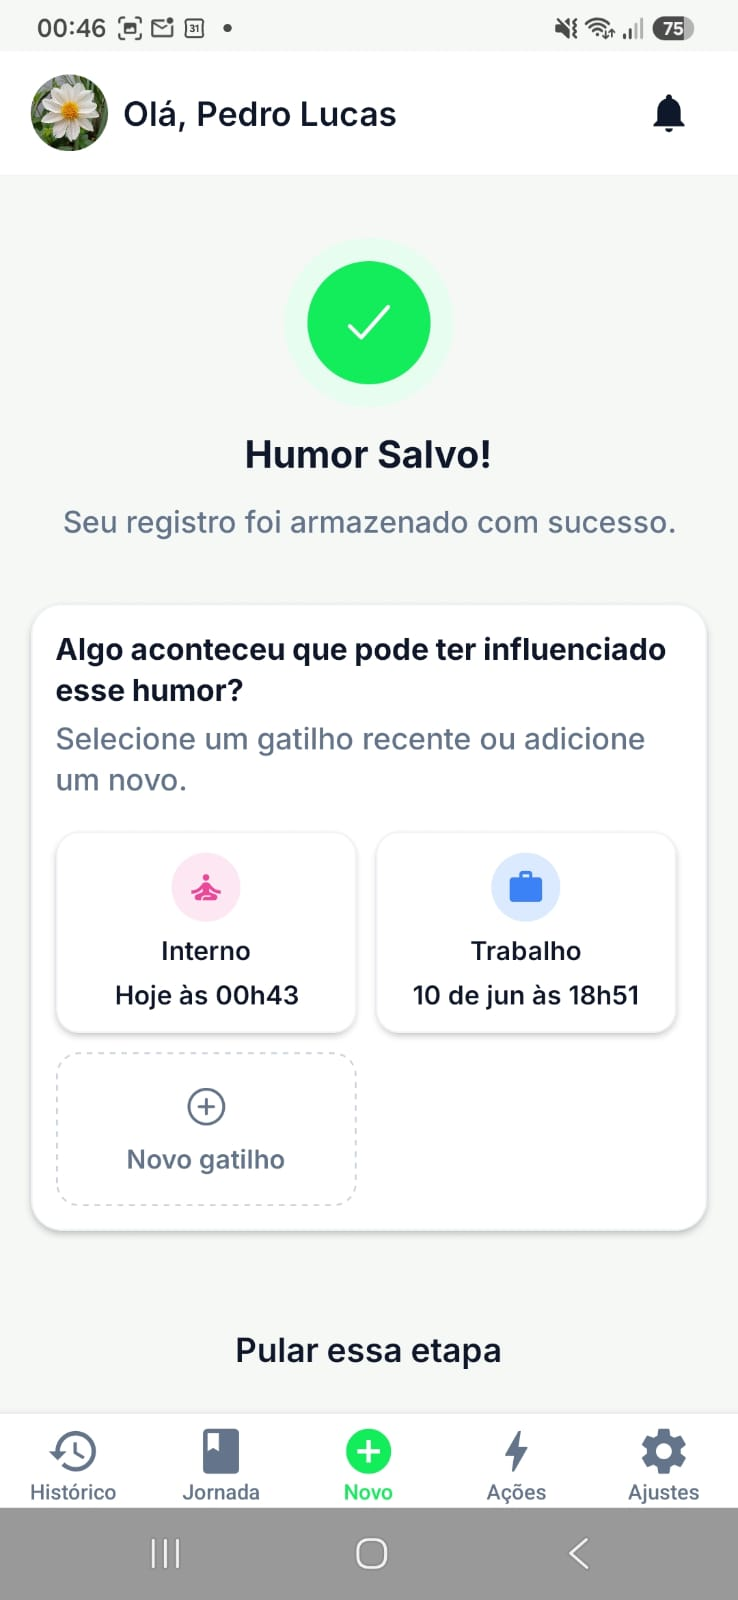
\includegraphics[width=0.70\textwidth,height=0.60\textheight,keepaspectratio]{screenshot-link-mood-with-trigger.jpeg}
\source{Elaborado pelo autor (2026)}
\end{figure}

Em seguida, o usuário pode indicar o impacto que aquele gatilho
exerceu sobre o registro de humor em questão. Novamente, trata-se de
uma estimativa subjetiva, sem pretensão de precisão.

\begin{figure}[H]
\centering
\caption{Avaliando o impacto de um gatilho no humor}
\label{fig:screenshot-assess-trigger-mood-impact}
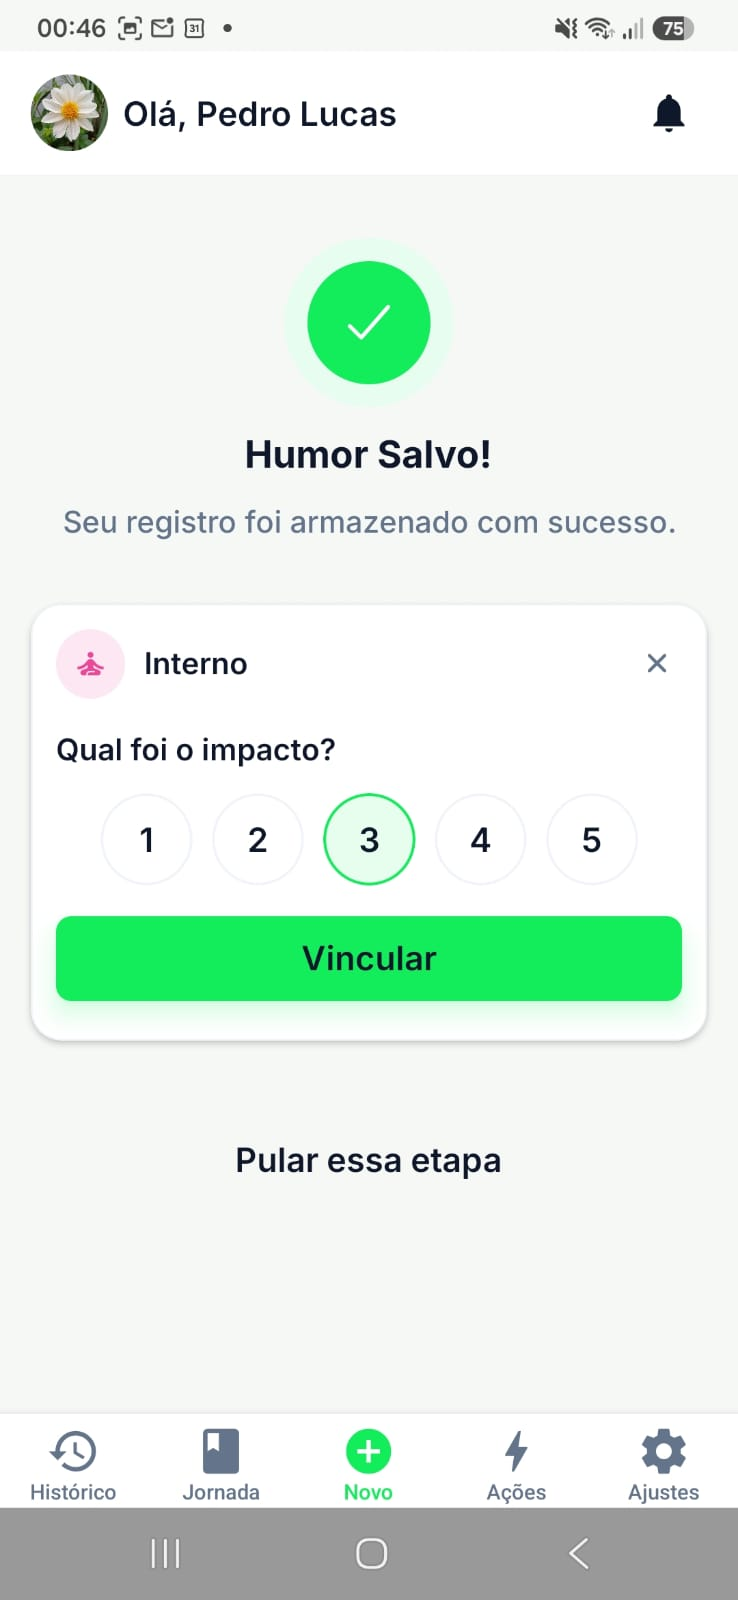
\includegraphics[width=0.70\textwidth,height=0.60\textheight,keepaspectratio]{screenshot-link-mood-assess-impact.jpeg}
\source{Elaborado pelo autor (2026)}
\end{figure}

Por fim, vale mencionar que, após esse processo, é enfileirado
internamente um \textit{background job} que recalcula, sob demanda, o
indicador de energia daquele dia, apresentado na figura
\ref{fig:screenshot-consulta-registros}. Diferentemente deste, os
indicadores semanais --- como a correlação entre sono e energia,
descrita na seção \ref{sec:insights} --- não são recalculados a cada
registro individual, sendo processados apenas pelo job semanal
agendado (seção \ref{sec:insights}).

\section{Indicadores}\label{sec:insights}

Nessa tela é apresentado um conjunto de indicadores construídos a partir
dos registros de humor, sono e gatilho do usuário. Diferente das demais
telas do aplicativo, que operam sobre dados em tempo real, os indicadores
são artefatos pré-computados: um \textit{worker} assíncrono (\textit{BullMQ})
percorre semanalmente todos os usuários ativos e enfileira, para cada
um, um conjunto de \textit{jobs} --- um por tipo de indicador --- que
processam a janela dos últimos sete dias e persistem o resultado em uma
tabela dedicada. Vale notar que nem todos os indicadores seguem esse
fluxo agendado: os indicadores diários (energia e sono) são recalculados
sob demanda, no momento em que o usuário registra um novo humor ou
sessão de sono, enquanto os indicadores semanais dependem
exclusivamente do \textit{job} de \textit{fan-out} de segunda-feira.

O aplicativo móvel apenas consulta esse resultado já
calculado, o que evita repetir cálculos custosos a cada abertura da tela
e desacopla a lógica analítica do restante da API.

\begin{figure}[H]
\centering
\caption{Tela de indicadores}
\label{fig:screenshot-insights}
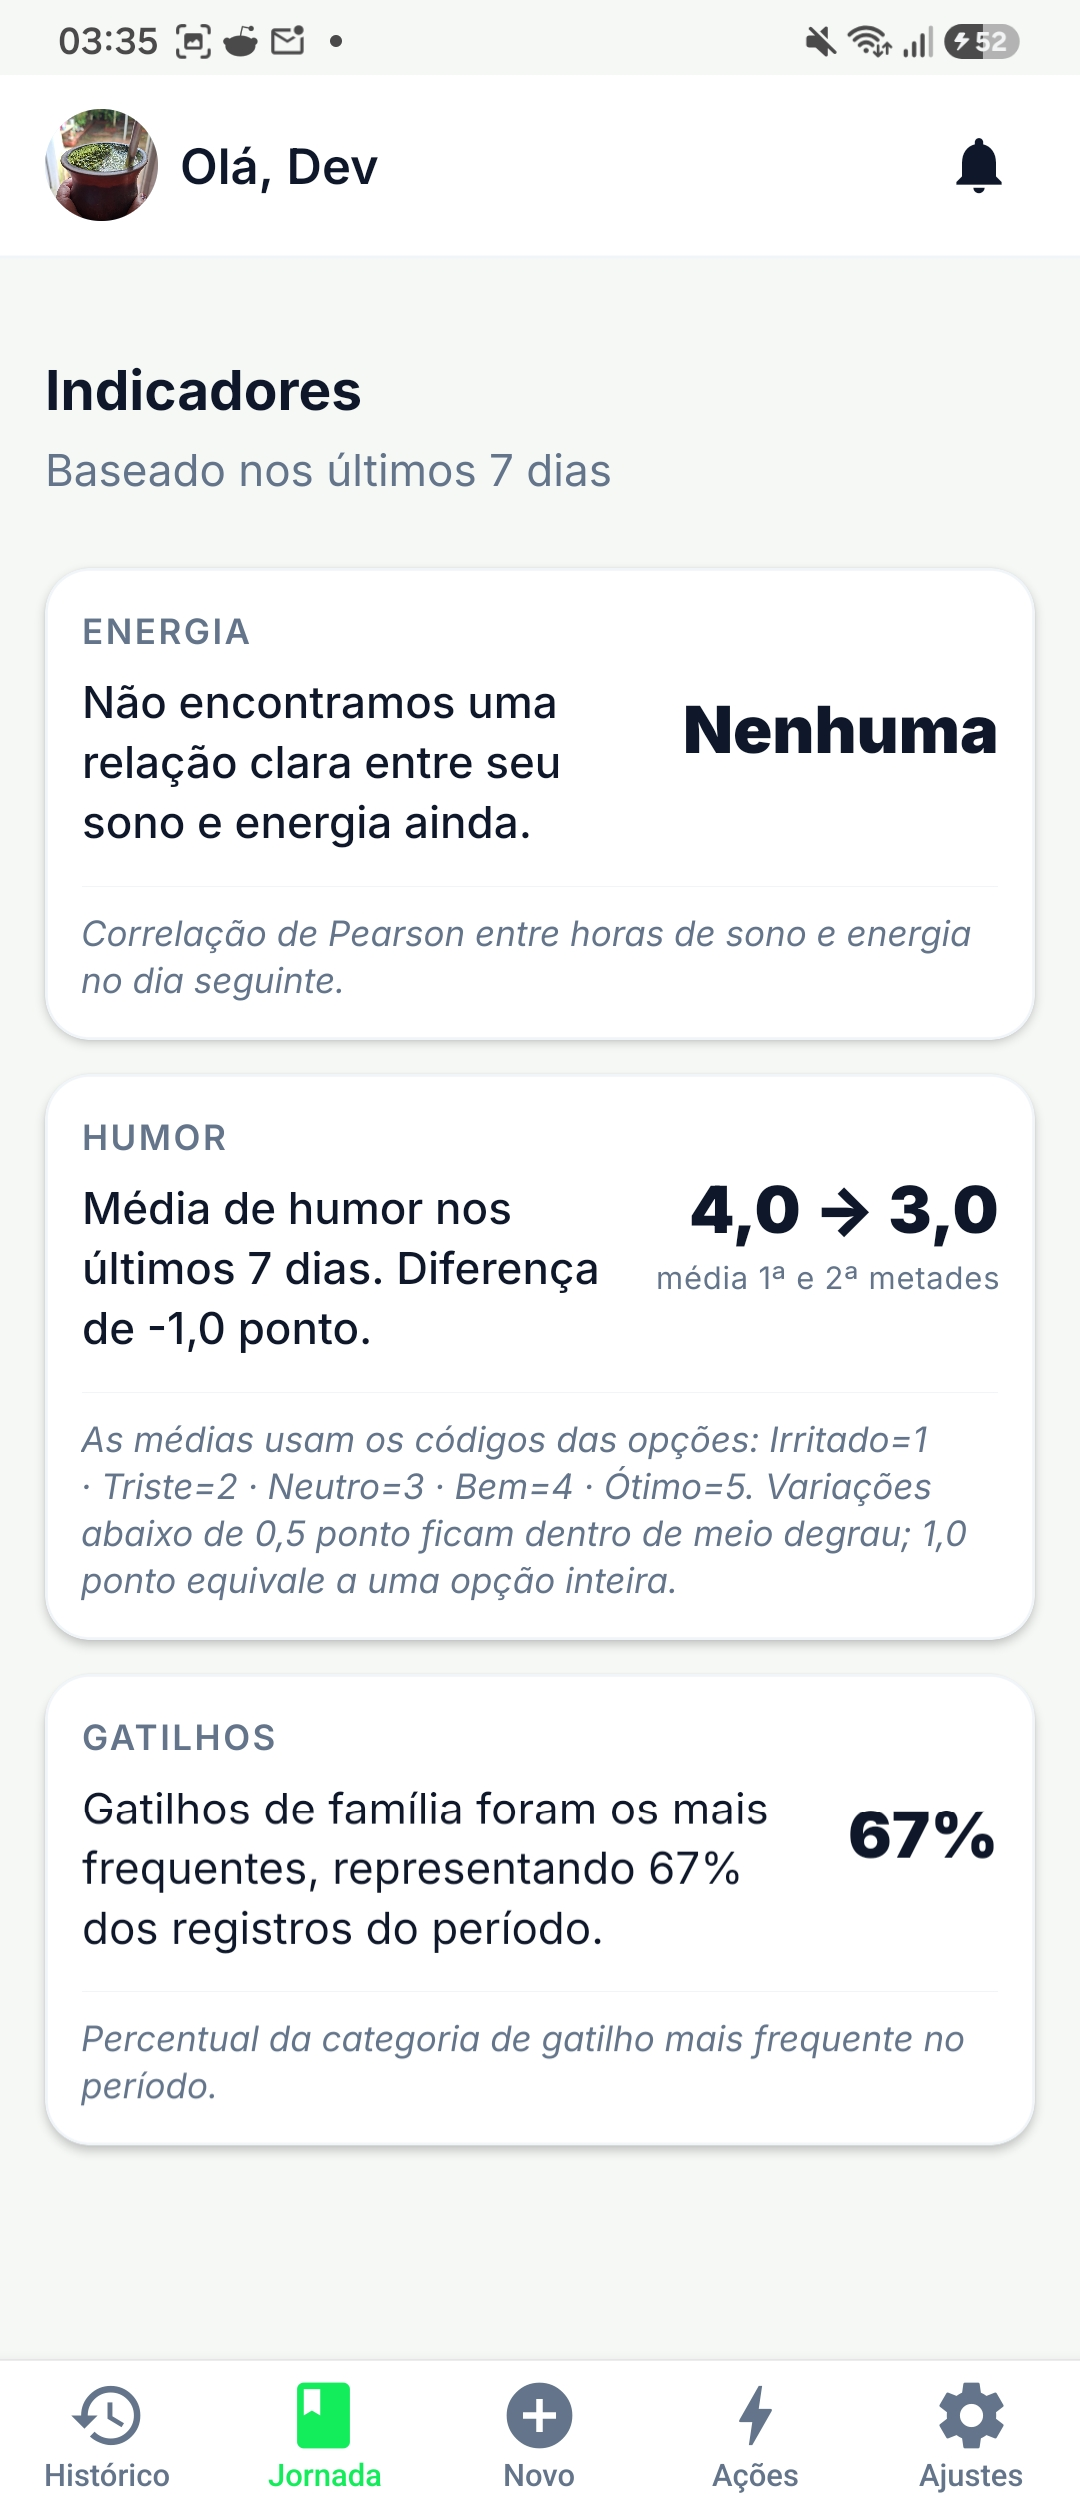
\includegraphics[width=0.70\textwidth,height=0.60\textheight,keepaspectratio]{screenshot-insights.jpeg}
\source{Elaborado pelo autor (2026)}
\end{figure}

% TODO: referenciar EMA / momentary assessment como justificativa da janela de 7 dias

São três os indicadores semanais exibidos: tendência de humor, correlação
entre sono e energia, e padrão de gatilhos.

\begin{itemize}
    \item \textbf{Tendência de humor}: compara a média de humor da
    primeira metade dos últimos sete dias com a da segunda metade,
    exibindo as duas médias na escala de 1 (Irritado) a 5 (Ótimo) e a
    diferença entre elas em pontos. Não há classificação automática de
    melhora, piora ou estabilidade: um ponto equivale a uma opção
    inteira, e variações abaixo de 0,5 ponto ficam dentro de meio
    degrau da escala. A leitura do restante fica a cargo do usuário.

    \item \textbf{Correlação entre sono e energia}: relaciona a duração
    do sono de uma noite com o nível de energia relatado na manhã
    seguinte, através do coeficiente de correlação de Pearson. Exige um
    mínimo de observações pareadas para ser calculado --- caso contrário,
    o indicador simplesmente não é exibido.

    \item \textbf{Padrão de gatilhos}: identifica a categoria de gatilho
    mais frequente na semana e expressa sua predominância como percentual
    do total de registros.
\end{itemize}

É intencional, na figura \ref{fig:screenshot-insights}, que o bloco de
``Energia'' apareça vazio: o cálculo da correlação depende da existência
simultânea de registros de sono \emph{e} de humor em quantidade mínima,
e no período retratado o usuário ainda não havia acumulado dados
suficientes de ambos os tipos. Optou-se por não exibir uma correlação
calculada com poucos pontos, preferindo comunicar a ausência de dado a
apresentar um número pouco confiável.

O bloco maior no topo da tela, o ``Resumo Semanal'', condensa os
indicadores mais centrais --- média de sono do período e um rótulo de
humor (``Estável'', no exemplo). Esse rótulo, no entanto, é o elemento
mais delicado de toda a funcionalidade. Embora exista uma fórmula capaz
de produzir uma classificação de estabilidade a partir da variância dos
registros de humor, atribuir esse tipo de afirmação a um usuário ---
especialmente em um aplicativo que é utilizado por pessoas com
Transtorno Afetivo Bipolar, para quem uma leitura equivocada de
``estabilidade'' pode mascarar justamente o início de um episódio ---
exige um embasamento mais cuidadoso do que uma regra estatística
simples. Por esse motivo, o rótulo apresentado nesta versão do
aplicativo é estático (não deriva de fato do cálculo de estabilidade) e
a funcionalidade pode ser inteiramente desabilitada pelo usuário nas
configurações. A decisão de manter ou não uma afirmação automatizada
desse tipo, e sob quais critérios, permanece um ponto em aberto que
mereceria revisão de literatura específica antes de ser tratado como
funcionalidade definitiva.

% TODO: literatura sobre riscos de auto-monitoramento automatizado de humor / mood-tracking apps e TAB

\section{Histórico}\label{sec:history-analysis}

Nessa tela é apresentado o histórico consolidado de registros de humor,
sono, gatilho e ações de cuidado (como sessões de terapia), organizados
cronologicamente e agrupados por dia, conforme a figura
\ref{fig:screenshot-history}. O usuário pode ainda filtrar a listagem por
categoria (``Humor'', ``Sono'', ``Gatilho'' e ``Ações de Cuidado''),
reduzindo o volume de informação exibida.

\begin{figure}[H]
\centering
\caption{Tela de Histórico}
\label{fig:screenshot-history}
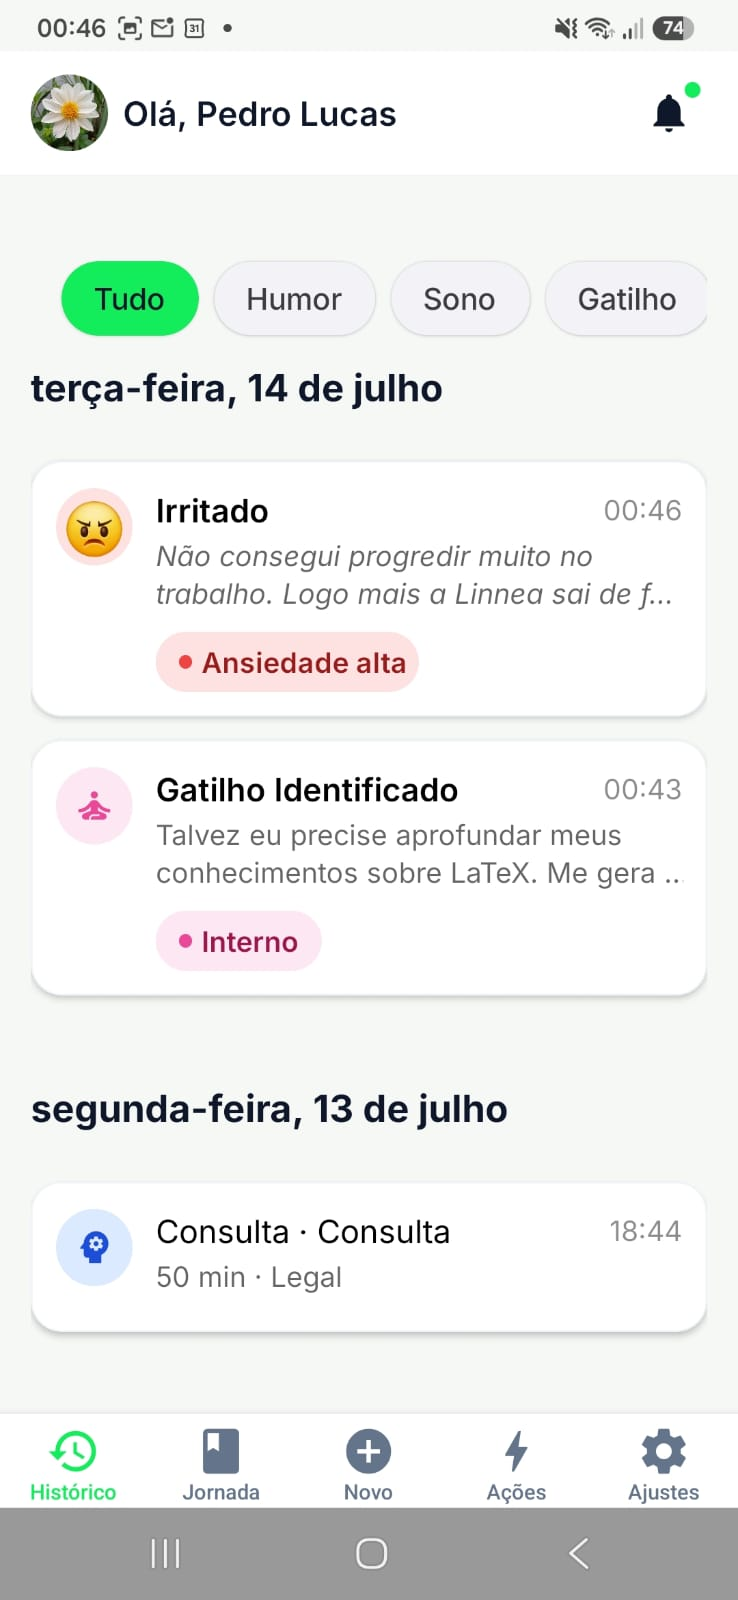
\includegraphics[width=0.70\textwidth,height=0.60\textheight,keepaspectratio]{screenshot-history.jpeg}
\source{Elaborado pelo autor (2026)}
\end{figure}

Os quatro tipos de dado residem em recursos distintos do banco, mas a
consolidação não acontece no aplicativo. Um único \textit{endpoint}
autenticado, \texttt{GET /history}, recebe \texttt{limit}, \texttt{cursor}
e \texttt{type} e devolve uma página já mesclada, na forma
\texttt{\{ items, nextCursor \}}. No servidor, cada uma das quatro tabelas
é consultada com o mesmo limite e o corte adequado ao seu tipo, e os
resultados são ordenados em conjunto, de modo que a ordem exibida pertence
à API, e não a uma composição de listas feita no dispositivo. Cada item é
a própria entidade acrescida de \texttt{kind}, que identifica o tipo, e de
\texttt{sortAt}, o instante usado para ordenar e agrupar, conforme o
código \ref{lst:history-card}.

\newpage

\begin{lstlisting}[caption={Formatos do histórico no servidor e no cartão da tela}, label={lst:history-card}]
export type HistoryItem =
  | (MoodEntry & { kind: "mood"; sortAt: Date })
  | (SleepRecord & { kind: "sleep"; sortAt: Date })
  | (Trigger & { kind: "trigger"; sortAt: Date })
  | (CareAction & { kind: "care_action"; sortAt: Date });

export interface HistoryPage {
  items: HistoryItem[];
  nextCursor: string | null;
}

export type HistoryCard = {
  id: string; // "<category>-<id>"
  category: HistoryCategory;
  subtype?: CareActionSubtype; // only for care actions
  timestamp: string; // ISO string, from sortAt
  title: string;
  summary: string;
  badge?: HistoryBadge;
  raw: MoodEntry | SleepRecord | Trigger | CareAction;
};
\end{lstlisting}

A ordenação total é decrescente por \texttt{sortAt}; em caso de empate,
crescente por \texttt{kind}, em uma ordem fixa; e, por fim, decrescente por
\texttt{id}. Humor, gatilho e ação de cuidado têm um momento próprio, que
serve como \texttt{sortAt}; o registro de sono é diário e não possui hora,
então o servidor o ancora ao meio-dia no fuso
\texttt{America/Sao\_Paulo}. O cursor é uma codificação \texttt{base64url}
de \texttt{\{ sortAt, kind, id \}} que o aplicativo não interpreta: apenas
a devolve na requisição seguinte, e a página começa estritamente depois do
registro que ela identifica. Trata-se de paginação por chave, e não por
deslocamento, porque o histórico cresce no topo: um deslocamento fixo
passaria a repetir ou a pular registros à medida que novos fossem
inseridos.

No aplicativo, um mapeador converte cada item no cartão exibido pela
tela --- um \texttt{HistoryCard}, que reaproveita os mesmos componentes
por categoria ---, e o instante exibido vem de \texttt{sortAt}, sem
recalcular a data a partir de cada registro. Os itens são então
reagrupados por dia, conforme visto na figura
\ref{fig:screenshot-history}, nos cabeçalhos ``terça-feira, 14 de julho''
e ``segunda-feira, 13 de julho''. Essa unificação é proposital:
ao invés de apresentar quatro telas separadas por tipo de dado, o
histórico busca reconstruir uma narrativa única do dia do usuário,
aproximando-se do princípio de \textit{Ecological Momentary Assessment}
já mencionado anteriormente --- o contexto de um registro de humor (por
exemplo, o gatilho ``Interno'' registrado três minutos antes, na mesma
figura) fica visualmente próximo do evento que possivelmente o motivou.

O cartão guarda o dado original na propriedade \texttt{raw}, permitindo
que a listagem redirecione o usuário para a tela de detalhe correta ao
tocar em um card, independentemente da categoria. Já a propriedade
\texttt{badge} reaproveita o mesmo mecanismo já descrito na seção de
indicadores: para um registro de sono, sinaliza se a duração foi
insuficiente; para um registro de humor, destaca a dimensão mais relevante
daquele registro (como ``Ansiedade alta'' na
figura \ref{fig:screenshot-history}); para um gatilho, indica sua
categoria, e assim por diante.

A lista é renderizada por uma \texttt{SectionList} virtualizada, que
monta apenas os cartões próximos à janela visível, e não todos os
registros de uma vez. As seções são reconstruídas a partir de todos os
itens acumulados após cada página, o que mantém os registros de um mesmo
dia sob um único cabeçalho ainda que a fronteira entre páginas caia no
meio do dia; os cabeçalhos, por sua vez, não permanecem fixos no topo
durante a rolagem, preservando o comportamento anterior. Ao se aproximar
do fim da lista, o aplicativo requisita a página seguinte. O filtro ativo
é enviado como o parâmetro \texttt{type}, e cada categoria mantém seu
próprio fluxo de cursor, de modo que trocar de filtro reinicia a partir
da página mais recente. O gesto de puxar para atualizar descarta o
acumulado e recomeça da primeira página; enquanto uma página carrega, um
indicador no rodapé sinaliza a espera, e uma falha oferece a ação de
tentar novamente em vez de se confundir com o fim do histórico.

\section{Exportação de Dados e Relatórios}\label{sec:export-report}

Além das telas de consulta e análise, o Nexo oferece duas formas de
levar os dados para fora do aplicativo: a exportação integral dos
registros, em formato aberto, e a geração de um relatório resumido em
PDF. Ambas materializam o princípio de soberania dos dados discutido nos
capítulos anteriores --- princípio reforçado pelo questionário, em que a
maioria dos respondentes atribuiu nota máxima à importância de ter
controle total sobre as próprias informações. A diferença entre as duas
reside no propósito: a exportação devolve a totalidade dos dados em um
formato legível e processável, enquanto o relatório condensa um período
específico em um documento pronto para ser guardado ou compartilhado com
um profissional de saúde.

A exportação é acionada na tela de configurações, na opção ``Exportar
Meus Dados''. Antes de disparar o processo, o aplicativo pede uma
confirmação e informa que o arquivo será enviado para o e-mail cadastrado
--- um lembrete explícito de que aquela operação retira dados do
dispositivo e os entrega por um canal externo.

% TODO: adicionar screenshot da tela de exportação (modal de confirmação)

Do ponto de vista técnico, a solicitação enfileira um \textit{job}
assíncrono na mesma infraestrutura de filas descrita na
seção~\ref{sec:insights}. O \textit{worker} percorre todas as entidades
associadas ao usuário --- perfil, humores e seus componentes, sono,
gatilhos e seus vínculos, ações de cuidado, medicamentos, consultas,
atividades e os indicadores já calculados --- e serializa cada uma em um
arquivo CSV próprio, com os rótulos traduzidos e os valores enumerados
convertidos para texto legível. Os arquivos são compactados em um único
\textit{zip}, acompanhados de um manifesto com a data de geração, e o
pacote é anexado a um e-mail enviado ao usuário; em caso de falha, um
e-mail de erro é disparado em seu lugar. O resultado é uma exportação
completa e portátil: nenhum campo é omitido ou agregado, de modo que o
usuário pode reimportar os dados em outra ferramenta ou auditá-los
diretamente --- alinhado à exigência de portabilidade levantada nos
requisitos não funcionais.

O relatório, por sua vez, é gerado sob demanda a partir da tela
``Relatório'', acessível também pelas configurações. O usuário escolhe um
período --- por meio de atalhos de 7, 30 ou 90 dias, ou um intervalo
personalizado limitado a 90 dias --- e aciona ``Gerar relatório''.

\begin{figure}[H]
\centering
\caption{Tela de geração de relatório}
\label{fig:screenshot-report}
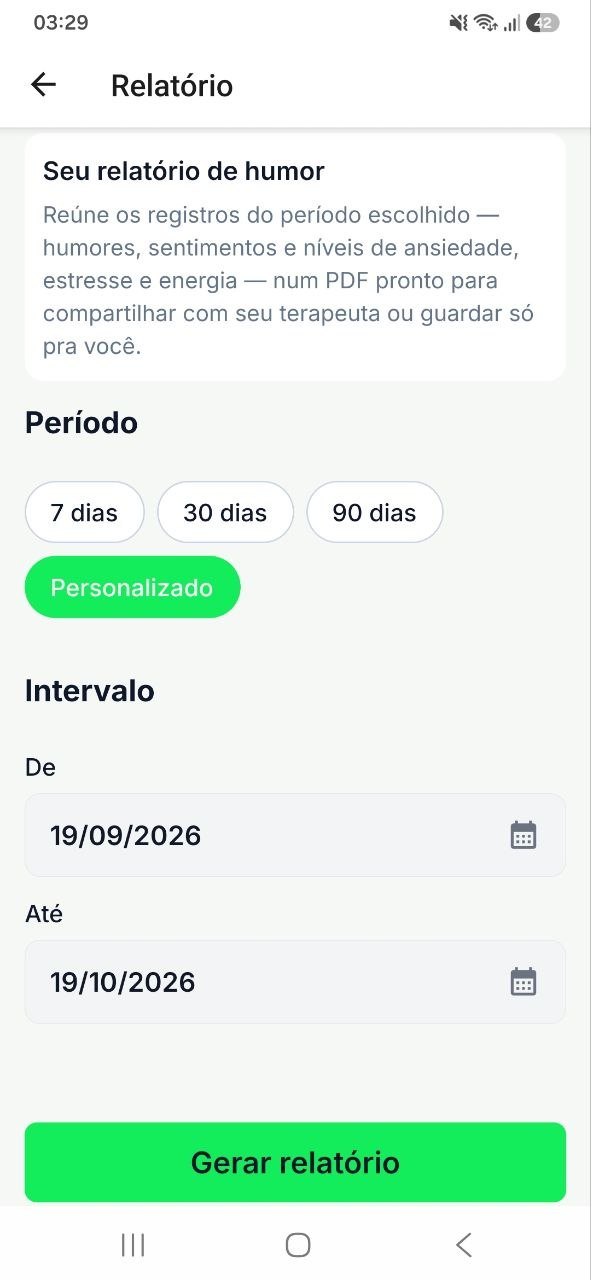
\includegraphics[width=0.70\textwidth,height=0.60\textheight,keepaspectratio]{screenshot-report-initial.png}
\source{Elaborado pelo autor (2026)}
\end{figure}

O servidor reúne os registros de humor do período e os renderiza em um
PDF intitulado ``Relatório de Humor e Bem-Estar'', produzido com
\textit{@react-pdf/renderer} e devolvido ao aplicativo, que o oferece
pela folha de compartilhamento nativa do sistema --- permitindo salvá-lo
ou enviá-lo a um terapeuta. O documento é dividido em duas páginas: a
primeira traz uma visão geral (total de \textit{check-ins}, humor
predominante e dias rastreados), a distribuição percentual de cada humor
e um mapa de calor diário; a segunda lista os sentimentos e emoções mais
frequentes, com a intensidade média, e o registro detalhado dos
\textit{check-ins}, com os níveis de ansiedade, estresse e energia.

Cabe registrar, contudo, que o relatório desta versão cobre apenas os
dados de humor. A intenção original era incorporar também o sono, as
atividades e os padrões de gatilho --- inclusive a correlação entre sono
e energia já calculada nos indicadores ---, mas essa ampliação foi
adiada para uma versão futura. Como consequência, o relatório atual
complementa, mas não substitui, a exportação integral: para uma visão
completa de todos os tipos de dado, o usuário ainda recorre ao
\textit{zip} de CSV.

\FloatBarrier
